\section{Visão geral do sistema}
\label{sec:visao-sistema}
O sistema consiste em uma aplicação experimental para receber e armazenar registros de auditoria, acompanhada de um ambiente de avaliação das formas de comunicação. Um registro descreve um fato ocorrido, sua origem, a entidade envolvida e o ator responsável. O processamento compreende validação, serialização determinística, cálculo de SHA-256 e persistência com unicidade por identificador. O sistema não executa a operação de negócio que originou o fato, como alterar um cadastro: apenas recebe sua representação.

O público-alvo compreende pesquisadores e estudantes que reproduzam os ensaios e profissionais que analisem os custos de comunicação síncrona e assíncrona. A aplicação cliente envia eventos; o pesquisador configura o ambiente e interpreta as evidências. Não se prevê, neste escopo, um produto corporativo de auditoria, gerenciamento de usuários, edição de registros persistidos ou integração com dados pessoais reais.

Na variante síncrona, a API HTTP valida o evento e solicita ao repositório sua persistência antes de responder. Na variante assíncrona, outra API valida o mesmo contrato e encaminha a mensagem ao produtor Kafka. Um consumidor recebe as mensagens do tópico e utiliza o mesmo processamento e repositório. PostgreSQL mantém os registros; Kafka intermedeia o fluxo assíncrono. O monitoramento e os cenários de carga constituem uma camada experimental de geração, coleta e análise, separada da função de registro.

As funcionalidades implementadas incluem recebimento HTTP, validação, hash determinístico, persistência idempotente, confirmação individual de publicação, consumo, retry limitado, DLQ, confirmação de offsets e consultas de prontidão e de registro. Scripts executam carga e consolidam logs, offsets, recursos e dados persistidos. Os quatro wireframes descrevem a interface de operação proposta; a comparação científica definitiva depende do protocolo e das repetições previstos no Capítulo~\ref{cap:metodo}. A Figura~\ref{fig:visao-geral} apresenta os componentes e a camada de avaliação.

\begin{figure}[htbp]
\centering
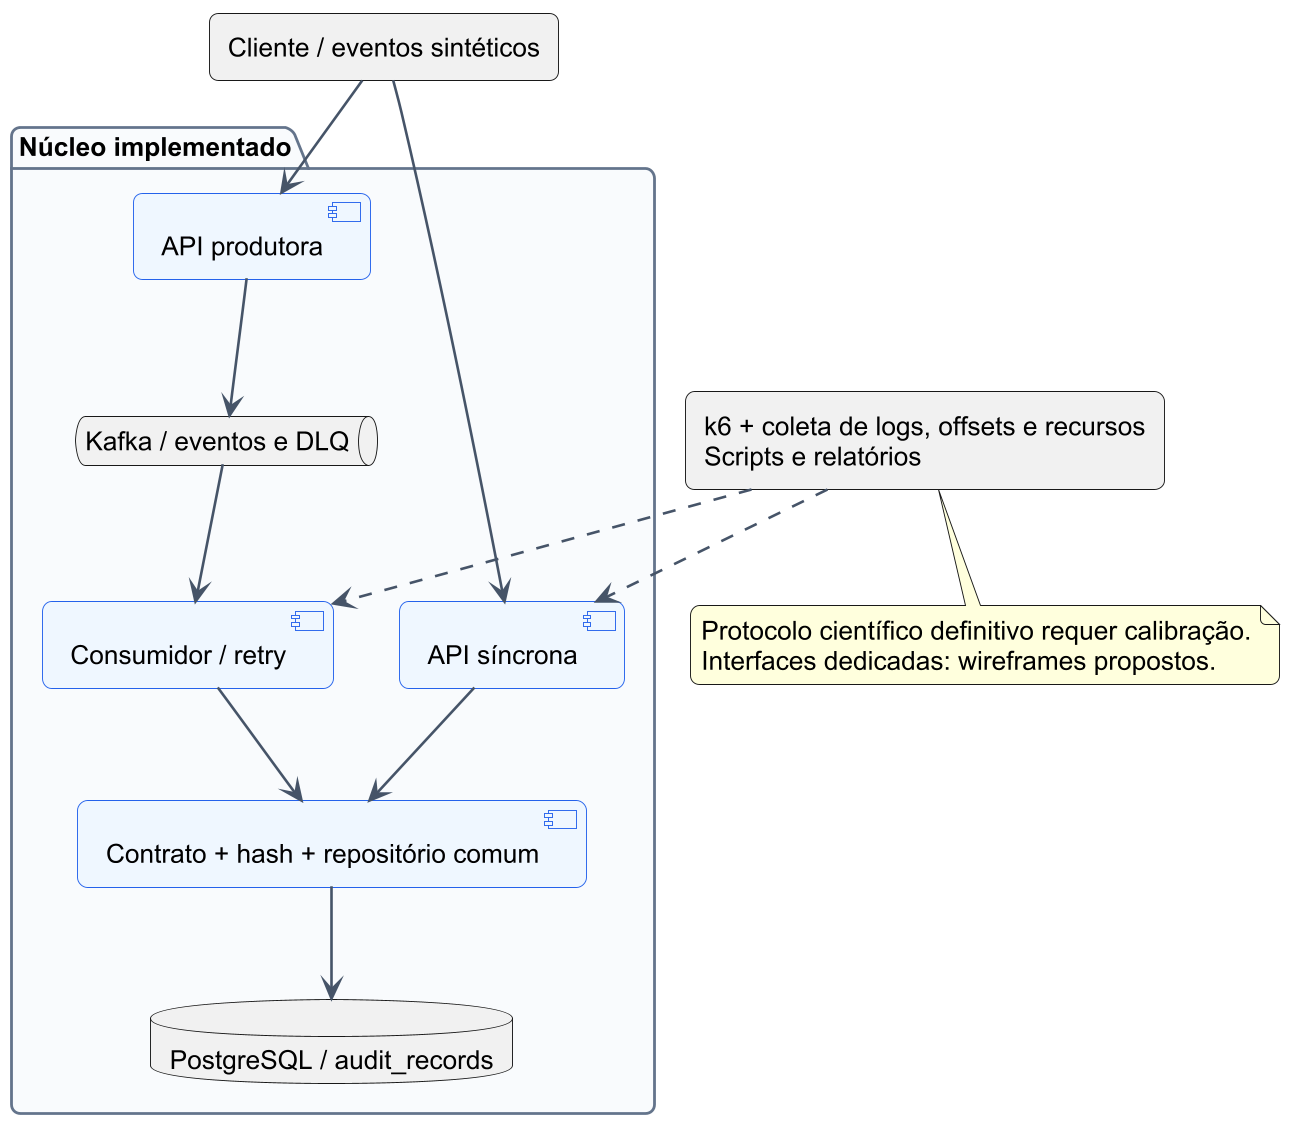
\includegraphics[width=0.95\textwidth,height=0.43\textheight,keepaspectratio]{Diagramas/plantuml/visao-geral.png}
\caption{Visão geral e delimitação do ambiente experimental}
\label{fig:visao-geral}
\fonte{Elaborado pelo autor (2026).}
\end{figure}

Nesta documentação, \textbf{implementado} indica que existe código para o comportamento descrito; a evidência dos testes e seu alcance são apresentados na Seção~\ref{sec:evidencias}. \textbf{Parcial} indica cobertura incompleta do requisito. \textbf{Planejado} identifica um componente ou procedimento ainda não implementado. Uma funcionalidade aprovada em teste não implica validação da hipótese científica.

A resposta \texttt{202 Accepted} sucede o ACK do broker e não significa que o registro já exista no PostgreSQL. Falhas de entrega podem produzir resultado incerto, enquanto falhas de consumo podem resultar em retry ou DLQ. A presença de uma mensagem na DLQ permite inspeção, mas não equivale a processamento concluído. O broker único limita a avaliação à topologia local, sem garantia de alta disponibilidade de cluster.

\textbf{Síntese.} As duas rotas executam o mesmo processamento e diferem na comunicação e nas condições de confirmação. O estado de cada requisito é vinculado ao código e às evidências, preservando a distinção entre validação funcional e comparação experimental.
